\documentclass[12pt]{report}

\usepackage[utf8]{inputenc}
\usepackage[T1]{fontenc}
\usepackage[francais]{babel}
\usepackage{SIunits}




\usepackage[a4paper,left=2cm,right=2cm,top=2cm,bottom=2cm]{geometry}
\usepackage{libertine}
\usepackage[pdftex]{graphicx}

\setlength{\parindent}{0cm}
\setlength{\parskip}{1ex plus 0.5ex minus 0.2ex}
\newcommand{\hsp}{\hspace{20pt}}
\newcommand{\HRule}{\rule{\linewidth}{0.5mm}}

\begin{document}
\begin{titlepage}
  \begin{sffamily}
  \begin{center}
    \textsc{\LARGE École Polytechnique de Louvain\\Université Catholique de Louvain}\\[2cm]
    \textsc{\Large LMECA 1120: Introduction au méthodes d'éléments finis}\\[1.5cm]
    \HRule \\[0.4cm]
    { \huge \bfseries Projet final: élasticité linéaire tridimensionnelle\\[0.4cm] }
    \HRule \\[0.4cm]
   \vfill
   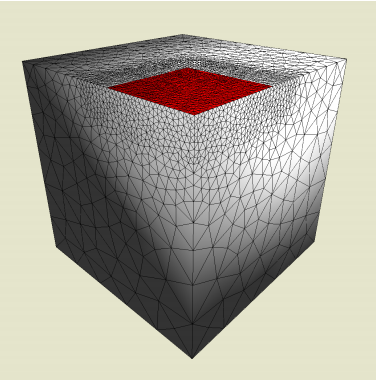
\includegraphics[scale=1]{cube}
   \vfill    
    \begin{minipage}{0.4\textwidth}
      \begin{flushleft} \large
        Boigelot \textsc{Simon}\\
        Nicol \textsc{Edward}\\
      \end{flushleft}
    \end{minipage}
    \begin{minipage}{0.4\textwidth}
      \begin{flushright} \large
        \emph{Professeur :} Vincent \textsc{Legat}\\
      \end{flushright}
    \end{minipage}
    \vfill
    {\large Mai 2015}
  \end{center}
  \end{sffamily}
\end{titlepage}

\section*{Obtention de la formulation faible}
Nous ne considèrerons dans ce rapport que la première équation donnée dans l'énoncé du projet. Il suffit d'appliquer exactement la même démarche aux deux dernières équations.\\ La méthode d'éléments finis est une méthode de résidus pondérés. La technique de Galerkin consiste à prendre les fonction de formes comme poids. Ainsi, l'équation peut être réecrite: $$ <\phi_{i} \frac{\partial{\sigma_{xx}}}{\partial{x}}> + <\phi_{i} \frac{\partial{\sigma_{xy}}}{\partial{y}}> + <\phi_{i} \frac{\partial{\sigma_{xz}}}{\partial{z}}>     = 0$$ En procédant à une intégration par partie, nous obtenons: $$ <\frac{\partial{\phi_{i}}}{\partial{x}} \sigma_{xx}> + <\frac{\partial{\phi_{i}}}{\partial{y}} \sigma_{xy}> + <\frac{\partial{\phi_{i}}}{\partial{z}} \sigma_{xz}> =  \ll \phi_{i}n_{x}\sigma_{xx} \gg +  \ll \phi_{i}n_{y}\sigma_{xy} \gg +  \ll \phi_{i}n_{z}\sigma_{xz} \gg $$ Le terme de droite étant nul vu les conditions homogènes que nous imposons  dans le problème. En remplacant $\sigma_{xx}$, $\sigma_{xy}$, $\sigma_{xz}$ par leur expression respective donnée dans l'énoncé et en posant $A = \frac{E}{1+\nu}$, $B = \frac{E\nu}{(1+\nu)(1-2\nu)}$, $C = \frac{E}{2(1+\nu)}$ nous obtenons maintenant:\\\\ $A<\frac{\partial{\phi_{i}}}{\partial{x}} \frac{\partial{u}}{\partial{x}}> + B<\frac{\partial{\phi_{i}}}{\partial{x}}\left(\frac{\partial{u}}{\partial{x}}+\frac{\partial{v}}{\partial{y}}+\frac{\partial{w}}{\partial{z}}\right)> + C<\frac{\partial{\phi_{i}}}{\partial{y}} \left(\frac{\partial{u}}{\partial{y}}+\frac{\partial{v}}{\partial{x}}\right)> + C<\frac{\partial{\phi_{i}}}{\partial{z}} \left(\frac{\partial{u}}{\partial{z}} + \frac{\partial{w}}{\partial{x}}\right)> = 0$\\\\
En tenant maintenant compte du fait qu'en toute généralité, $\frac{\partial{a}}{\partial{x}} = \sum_{j=1}^{4}A_{j}\frac{\partial{\phi_{j}}}{\partial{x}}$, nous pouvons réecrire l'équation ci-dessus sous sa forme finale:\\\\
$$\sum_{j=1}^{4}U_{j}\left[\left(A+B\right)<\frac{\partial{\phi_{i}}}{\partial{x}}\frac{\partial{\phi_{j}}}{\partial{x}}>+C<\frac{\partial{\phi_{i}}}{\partial{y}}\frac{\partial{\phi_{j}}}{\partial{y}}>+C<\frac{\partial{\phi_{i}}}{\partial{z}}\frac{\partial{\phi_{j}}}{\partial{z}}>\right]$$ $$+$$ $$\sum_{j=1}^{4} V_{j}\left[B<\frac{\partial{\phi_{i}}}{\partial{x}}\frac{\partial{\phi_{j}}}{\partial{y}}>+C<\frac{\partial{\phi_{i}}}{\partial{y}}\frac{\partial{\phi_{j}}}{\partial{x}}>\right]$$ $$+$$ $$\sum_{j=1}^{4}W_{j}\left[B<\frac{\partial{\phi_{i}}}{\partial{x}}\frac{\partial{\phi_{j}}}{\partial{z}}>+C<\frac{\partial{\phi_{i}}}{\partial{z}}\frac{\partial{\phi_{j}}}{\partial{x}}>\right]$$ $$=$$ $$0$$
En procédant exactement de la même manière avec les deux dernières équations du problème, nous avons pu déterminer entièrement la formulation discrète du problème.


\end{document}